\documentclass[12pt]{article}
\usepackage{graphicx}
\usepackage[margin=0.8in]{geometry}
\usepackage{color, colortbl}
\usepackage{listings}

\definecolor{LightCyan}{rgb}{0.88,1,1}
\definecolor{LightRose}{rgb}{1,0.88,0.88}
\definecolor{LightGreen}{rgb}{0.88,1,0.88}
\definecolor{DarkGreen}{rgb}{0.10,0.40,0.10}
\definecolor{listinggray}{gray}{0.9}
\definecolor{lbcolor}{rgb}{0.9,0.9,0.9}

\lstset{
    backgroundcolor=\color{lbcolor},
    tabsize=4,
  language=C++,
  captionpos=b,
  tabsize=3,
  frame=lines,
  numbers=left,
  numberstyle=\tiny,
  numbersep=5pt,
  breaklines=true,
  showstringspaces=false,
  basicstyle=\footnotesize,
%  identifierstyle=\color{magenta},
  keywordstyle=\color[rgb]{0,0,1},
  commentstyle=\color{DarkGreen},
  stringstyle=\color{red}
  }


\title{High Performance Output Data Format for Nuclear Physics}
\author{Gagik Gavalian}
\date{May 2017}

\begin{document}

\begin{titlepage}
\maketitle
\begin{abstract}
This document describes a new data format used in nuclear physics community.
The data format was developed with specific goals to ease of use in multi-thread 
applications and for easy data distribution and reduction.
\end{abstract}
\end{titlepage}

\section{Introduction}

The High Performance Output (HIPO) data format was developed at Jefferson Lab
for storing experimental as well as DST data from physics runs. The file format
was designed agnostic to what data will be stored inside. On high level the file
is divided into chunks (we call them records) of data each of them containing N number
of events. Each chunk has it's own index table which points to specific event in the
chunk, and a data buffer which can be written in compressed or un-compressed from.
4 data buffer modes are supported: uncompressed, compressed with GZIP, compressed
with LZ4 (fast compression) and compressed with LZ4 (best compression). Depending
on the situation differen compressions can be used. GZIP provides the best compression
ratio but it is slow in compression time and decompression time. LZ4 is generally much
faster for both modes (fast and best), but yields to lower compression ratio. One thing 
to consider is that decompression of LZ4 is much faster than GZIP, so in our applications
we usually use LZ4-best mode.


\section{File structure}

HIPO file consists of a header describing parameters of the file such as version and the 
modes used in creating the file, header record containing dictionary for the file (more on
dictionaries in the next sections), followed by data chunks appended back to back.
The structure of the file is shown on Figure~\ref{FILE::STRUCTURE}.

%\begin{figure}[!ht]
%\begin{center}
%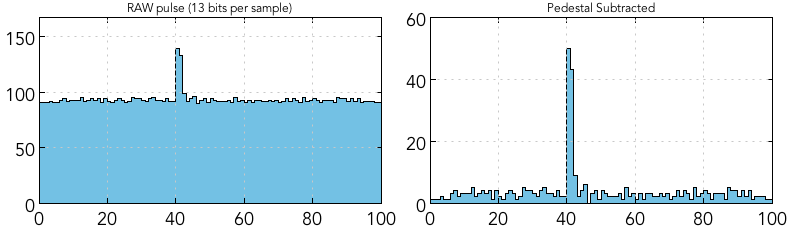
\includegraphics[width=6in]{pics/fadc_pulse_reduction.png}
 %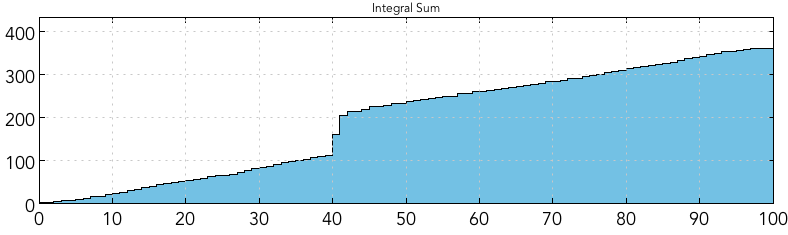
\includegraphics[width=6in]{pics/fadc_pulse_summ.png}
 %\caption {}
 %\label{FADC_PULSE}
%\end{center}
%\end{figure}

The header part of the file can contain several buffers, defined by user at the time 
when file is opened. By default there are two buffers that are present in the header
are dictionary buffer and record index buffer. Both of those can be empty if user did 
not provide them (more on record indexing in the next sections).

\section{Data Records}

Data record is a chunk of data within the file containing variable size events. The idea
is to have events grouped together for better compression and faster indexing of the file.
When reading the file sequentially each record is loaded into the memory and events are read
in sequence, once end of the record is reached, the next record is loaded. 
The record size can vary depending on application, usually when opening file writing user
can specify desired maximum record size (in bytes) or desired maximum events to be written 
in one record. Fine tuning of this numbers are dependent on the application. By default, the
file writer sets maximum size for the record to be 8~Mb, and maximum number of events
to $10^6$. 

The following example code shows how to create a record and populate it with events.

Example:

\begin{lstlisting}[language=C++,directivestyle={\color{black}}
                   emph={int,char,double,float,unsigned},
                   emphstyle={\color{blue}}]
 #include<stdio.h> 
 #include<iostream>
 #include "record.h"
 
 int main()
 {
    int nevents = 20;
    hipo::record record;
    for(int i=0; i < nevents; i++){ 
        int vsize = rand()%25 + 5;  // random number 5-30
        int value = rand()%255;     // random number 0-255
        std::vector<char> vec;
        vec.resize(vsize,value); 
        record.addEvent(vec);
    }
    std::vector<char> buffer = record.build(); // buffer containing encoded record
    return 0; 
 }
\end{lstlisting}

The example code creates a record and fills it with variable number arrays filled with random
numbers. Then returns packed representation of record that can be appended to the file.
In practice the file writer will take care of building the buffer and appending it to the file.
 
\section{Data Events}

The HIPO file and record are agnostic to the event structure stored inside, so it is up to the
user to handle the event parsing. The library provides a standardized event buffers that can be 
used to store arrays of specific types in an event tagged by two numbers called "group" and 
"item". The presence of two numbers gives ability to group relevant arrays together and
read them at once as part of one object. Events then are digitized into a buffer of chars 
to be appended to the record. 

Example:

\begin{lstlisting}[language=C++,directivestyle={\color{black}}
                   emph={int,char,double,float,unsigned},
                   emphstyle={\color{blue}}]
 #include<stdio.h> 
 #include<iostream>
 #include "record.h"
 #include "event.h"
 
 int main()
 {
    int nevents = 20;
    hipo::record record;
    hipo::event  event;
    for(int i=0; i < nevents; i++){ 
        int   vsize  = rand()%25 + 5;  // random number 5-30
        int   ivalue = rand()%16567;  // random number 0-16567
        float fvalue = (rand()%32567)/12.7;  //0-32567 divided by 12.7
        std::vector<int> vec_i(vsize,ivalue);
        std::vector<float> vec_f(vsize,fvalue);
        event.reset();
        event.appendNode(24, 1, vec_i); // group=24, item=1 type=integer
        event.appendNode(25, 2, vec_f); // group=25, item=2 type=float
        record.addEvent(event);
    }
    std::vector<char> buffer = record.build(); // record buffer
    return 0; 
 }
\end{lstlisting}

The example code creates two arrays of same size, one integer on float, and fills with
random numbers, then appends them to an event object each tagged with their group 
number and item number, then writes the event to the record. 

\end{document}
